O jogo Wolkenkratzer, também conhecido como Skyscrapers, é um quebra-cabeça que consiste em um tabuleiro quadrado de lado N com casas que devem ser preenchidas por números de 1 a N -- em alguns puzzles são permitidos espaços em branco junto de valores de 1 a N-1 -- que não podem ser repetidos entre linhas ou entre colunas (como no famoso Sudoku).
Em torno do tabuleiro são colocadas algumas restrições que representam o número de prédios que poderiam ser vistos por um observador naquela posição que olhasse na direção do tabuleiro.
Assim, cada número colocado em uma casa do tabuleiro representa um prédio daquela altura que encobre prédios vizinhos de menor altura em cada direção.

\begin{figure}[!htbp]
  \centering
  \begin{subfigure}[t]{0.45\textwidth}
    \centering
    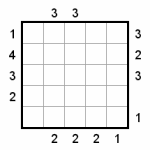
\includegraphics[width=0.8\linewidth]{empty}
    \caption{Estado inicial do \textit{puzzle}.}
  \end{subfigure}
  \begin{subfigure}[t]{0.45\textwidth}
    \centering
    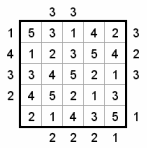
\includegraphics[width=0.8\linewidth]{solved}
    \caption{Solução dessa instância do jogo.}
  \end{subfigure}
  \caption{Exemplo de instância do jogo Wolkenkratzer.}
  \label{fig:example}
\end{figure}

A implementação do \textit{puzzle} em Prolog é simples: basta expressar as regras do quebra-cabeça e a relação das restrições (número de prédios observados a partir das bordas) com o tabuleiro inicialmente livre.
Utilizamos uma lista de listas para representar o tabuleiro e uma tupla de listas para representar as restrições em cada uma das quatro bordas, onde um valor $0$ é usado para indicar que não há restrição (em branco).
Além disso, recebemos um parâmetro para indicar a altura máxima que um prédio pode tomar e se é ou não necessário conferir as diagonais do tabuleiro (algumas instâncias requerem que não hajam repetições nas diagonais).

\begin{minted}[style=mannie]{prolog}
/* solves an instance of the skyscrapers puzzle defined by given constraints
  (0s are ignored), maximum building height and the option to check diagonals */
wolkenkratzer(Board, (Upper, Left, Bottom, Right), Max, DiagCheck) :-
    %% continua ...
\end{minted}

Primeiramente conferimos o tamanho do tabuleiro (e se as restrições possuem um tamanho compatível com o mesmo).
Logo, é possível delimitar o intervalo em que se encontrarão os valores de alturas dos prédios nas células do tabuleiro, o que é feito através da restrição \textit{ins}.

\begin{minted}[style=mannie]{prolog}
    %% ...
    
    % for a NxN board, each list of constraints has N values
    length(Board, N),
    length(Upper, N),
    length(Left, N),
    length(Bottom, N),
    length(Right, N),

    % cells can be filled with an integer value in the range [Min,Max]
    Min is 1 - (N - Max),
    Min >= 0,
    flatten(Board, Cells),
    Cells ins Min..Max,
    
    %% ...
\end{minted}

Em seguida adicionamos a restrição de que cada linha possui elementos distintos, o mesmo valendo também para cada coluna.
Obtemos também uma versão invertida das linhas e colunas do tabuleiro, o que será útil para aplicar as restrições de todas as bordas.

\begin{minted}[style=mannie]{prolog}
    %% ...
    % rows dont repeat values and neither do columns
    Rows = Board,
    transpose(Rows, Columns),
    maplist(all_distinct, Rows),
    maplist(all_distinct, Columns),
    maplist(reverse, Rows, ReversedRows),
    maplist(reverse, Columns, ReversedColumns),
    %% ...
\end{minted}

Quando for necessário, verifica-se também se os elementos nas diagonais são distintos.
Note que o metapredicado \textit{maplist} foi muito útil para tornar o código curto e expressivo.

\begin{minted}[style=mannie]{prolog}
    %% ...
    % sometimes, diagonals need to be distinct as well
    diagonal_(DiagCheck, Rows, ReversedRows),
    %% ...
    
% auxiliary predicate that checks both wolkenkratzer diagonals only if needed
diagonal_(false, _, _).
diagonal_(true, Rows, ReversedRows):-
    diagonal(Rows, MainDiag), all_distinct(MainDiag),
    diagonal(ReversedRows, SecondDiag), all_distinct(SecondDiag).

% extracts main diagonal from a list of lists
diagonal(Rows, Diag) :-
    length(Rows, N), range(0, N, Indices), maplist(nth0, Indices, Rows, Diag).
\end{minted}

Assim, basta verificar se o número de prédios observados do ponto de vista de cada posição na borda do tabuleiro respeita a restrição fornecida (se diferente de zero).
Os predicados da biblioteca \textit{clpfd} são utilizados para garantir que as soluções do programa levem em conta as regras do jogo, onde o mecanismo de \textit{backtracking} de Prolog tenta fixar variáveis nas células do tabuleiro e falha sempre que os valores neste deixam de respeitar as restrições aplicadas anteriormente.

\begin{minted}[style=mannie]{prolog}
    %% ...

    % check if all constraints are met
    maplist(skyscrapers, Rows, Left),
    maplist(skyscrapers, ReversedRows, Right),
    maplist(skyscrapers, Columns, Upper),
    maplist(skyscrapers, ReversedColumns, Bottom),

    % collapse cell domains into single values
    maplist(label, Board).


% counts the number of visible skyscrapers on a given sequence
skyscrapers(_, 0).
skyscrapers([0|Rest], Constraint) :- skyscrapers(Rest, 0, Constraint, 0).
skyscrapers([First|Rest], Constraint) :-
    First #> 0, skyscrapers(Rest, First, Constraint, 1).

/* checks whether the number of visible skyscrapers in given sequence satisfies
   a constraint, starting with some max height and a previous count */
skyscrapers([], _, Constraint, Constraint).
skyscrapers([First|Rest], Max, Constraint, Seen) :-
    (First #> Max, Num #= Seen + 1, skyscrapers(Rest,First,Constraint,Num));
    (First #=< Max, skyscrapers(Rest,Max,Constraint,Seen)).
\end{minted}

O código mostrado já é suficiente para obter todas as soluções de instâncias quaisquer de Wolkenkratzer.
Entretanto, tabuleiros maiores evidenciam que o mecanismo de busca não é ótimo, com tempos de computação na ordem de dezenas de minutos para obter uma solução mais difícil.
Sendo assim, aplicamos algumas regras -- observadas ao jogar o jogo -- que podem ser aplicadas para reduzir as possibilidades consideradas pelo sistema de tentativa e erro.

\begin{minted}[style=mannie]{prolog}
    %% ...
    
    % apply pruning
    maplist(pruned(Min,Max), Rows, Left),
    maplist(pruned(Min,Max), ReversedRows, Right),
    maplist(pruned(Min,Max), Columns, Upper),
    maplist(pruned(Min,Max), ReversedColumns, Bottom),
    
    %% ...
    % check if all constraints are met
    %% ...
\end{minted}

É fácil perceber que uma restrição com o maior valor permitido implica uma sequência crescente de valores, assim como uma restrição de um único prédio pode ser resolvida de imediato com o prédio mais alto na célula adjacente.
Outra regra implementada consiste em encontrar um limitante superior na linha sobre a qual uma restrição se aplica, partindo do princípio de que valores mais altos devem estar mais longe das bordas para que seja possível observar mais prédios no tabuleiro.

\begin{minted}[style=mannie]{prolog}
%% applies pruning laws to further constrain value domains
% zero restrictions are ignored
pruned(_, _, 0).

% when tip is 1 and no parks are allowed, first cell is N
pruned(1, N, [N|_], 1).

% when tip is 1 and parks are allowerd, first cell is either Max or 0
pruned(0, Max, [First|_], 1) :- First #= Max; First #= 0.

% when tip is N, line is [1..N] (no parks)
pruned(1, N, Sequence, N) :- End #= N + 1, range(1, End, Sequence).

% when tip is some K, apply an upper bound to the whole line
pruned(_, N, Line, Tip) :- pruned_(N, Line, Tip).
pruned_(_, _, 0).
pruned_(_, [], _).
pruned_(N, [First|Rest], Tip) :-
    K is Tip - 1, First #=< N - K, pruned_(N, Rest, K).
\end{minted}

A adição dessas regras simples trouxe melhorias imediatamente perceptíveis à performance do programa, sendo possível (em alguns casos) inclusive fixar valores no tabuleiro somente através delas.
Todavia, após a inclusão desses predicados, o programa passou a fornecer múltiplas soluções iguais à uma mesma consulta.
